\section{Software}
Die Steuerung der Segel soll durch zwei verteilte Systeme erfolgen, die über eine Ethernet-Verbindung miteinander kommunizieren. Die Idee dahinter ist, die Berechnungen für die Ausrichtung der Segel in Abhängigkeit der Windstärke und -Richtung (Controllino) von der hardwarenahen Verarbeitung der Sensoren und Aktuatoren (stm32) logisch zu trennen. \\
Die vorliegende Arbeit konzentriert sich dabei lediglich auf das System der Sensoren und Aktuatoren, welches mit dem stm32 realisiert wurde. Die Aufgabe dieses Systems ist, zunächst die Linearführung zu kalibrieren, damit die aktuelle Position korrekt ermittelt werden kann. Außerdem soll über die Buttons am Gehäuse und zusätzlich über einen Webserver eine manuelle Steuerung ermöglicht werden. Während des Automatikbetriebs geschieht ein regelmäßiger Austausch aller relevanter Daten über eine REST basierte Schnittstelle. Dies beinhaltet u.A. die Information über aktuelle Windbedingung, Position der Segel, eventuelle Fehlerzustände (z.B. Motorfehler oder Überstrom) und daraus resultierende Befehle zur Anpassung der Segelstellung.
Für die Implementierung wurde die Software in komponentenorientierte Module eingeteilt:

\begin{figure}[H]
	\centering
	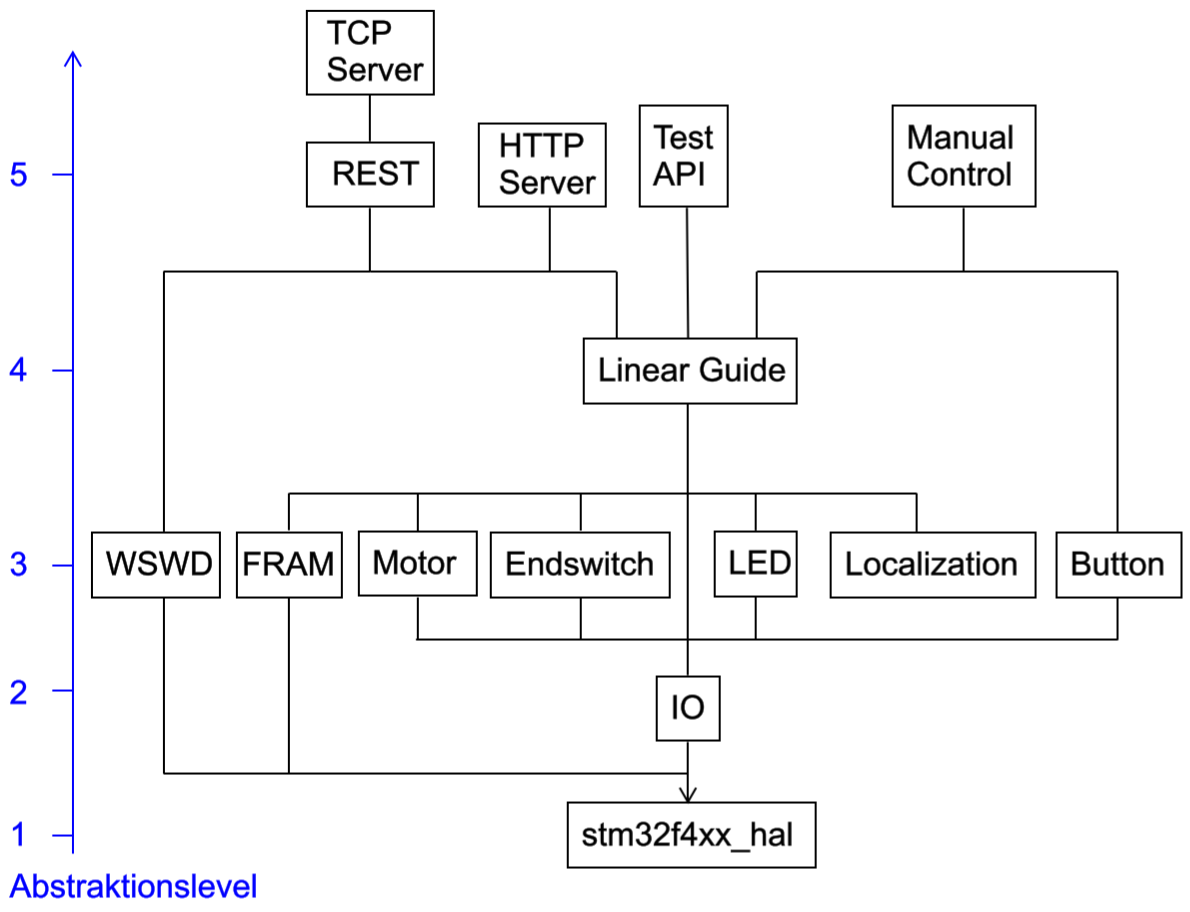
\includegraphics[width=0.6\linewidth]{images/Software/Modulestructure.png}
	\caption{Software Modulstruktur}
	\label{fig:modulestructure}
\end{figure}
\noindent
Abbildung \ref{fig:modulestructure} zeigt abwärtsgerichtet, wie die einzelnen Module aufeinander zugreifen. Auf unterster Abstraktionsebene laufen jegliche Operationen über die Standardbibliothek des Mikrocontrollers \verb|stm32f4xx\_hal|. Darüber liefert das \verb|IO|-Modul ein Set aus Hilfsfunktionen und -Strukturen für den allgemeinen Zugriff auf die GPIO-Pins und zum Auslesen analoger Messwerte der einzelnen Sensoren. Ebene drei umfasst hauptsächlich Module, welche alle relevanten Funktionalitäten der physischen Teilkomponenten des Systems implementieren, wie z.B. das Anemometer \verb|WSWD| oder der \verb|Motor|. Einige davon greifen dabei auf das \verb|IO|-Modul zu, wobei der allgemeine GPIO-Zugriff von einer spezifischen Funktion eingekapselt wird, wie z.B. das Einschalten einer LED im Falle des \verb|LED|-Moduls. Eine Ausnahme ist das \verb|Localization|-Modul, welches keine physische Komponente darstellt, sondern einige Hilfsfunktionen zur Kalibrierung und Positionsberechnung bereitstellt. Während die Module bis Ebene drei überwiegend allgemeingültig entworfen sind, enthält das \verb|Linear Guide|-Modul anwendungsspezifische Funktionen. Als zentrales Element bildet dieses ein High-Level Interface zur Verwendung der Teilkomponenten \verb|FRAM|, \verb|Motor|, \verb|Endswitch|, \verb|LED|, \verb|Localization| und \verb|IO|. Die Module der obersten Abstraktionsebene bilden die direkten Schnittstellen zur Außenwelt. Das \verb|Manual Control|-Modul ermöglicht die manuelle Steuerung der Linearführung über die User-Buttons am Gehäuse und insbesondere die Umsetzung des Kalibrierungsprozesses. Auf der anderen Seite kann das System auch durch einen HTTP Webserver überwacht und gesteuert werden. Außerdem werden im \verb|REST|-Modul die Anfragen des Controllinos über die \verb|TCP Server|-Verbindung verarbeitet, wie bereits oben erwähnt. Zuletzt wurde ein \verb|Test|-Modul implementiert, dass die Funktionalitäten der Module auf Ebene drei verifiziert. Dazu wurde ein einfaches Batch-Skript geschrieben, das die einzelnen Testcases auflistet und die Auswahl über UART an den  Mikrocontroller sendet, sodass im \verb|Test|-Modul eine entsprechende Funktion ausgeführt wird.\\In den nachfolgenden Abschnitten wird genauer auf einige Module eingegangen, beginnend mit dem untersten Abstraktionslevel.

\subsection{IO-Modul}
Dieses Modul soll den lesenden und schreibenden Zugriff auf jegliche GPIO-Pins erleichtern, die zur Kontrolle jeglicher Steuerelemente angeschlossen wurden. Allgemein besteht das System aus analogen und digitalen Sensoren bzw. Aktuatoren. Für jede Form wurde eine repräsentative Struktur definiert, in der alle relevanten Daten zusammengefasst werden.
\subsubsection{Digitale Pins}
Für digitale Ein- und Ausgänge wurde eine gemeinsame Struktur \verb|IO_digitalPin_t| definiert:
\begin{lstlisting}[language=C, caption={Struktur für digitale Pins}, label={lst:digitalPin}]
typedef struct {
	GPIO_TypeDef *GPIOx;
	uint16_t GPIO_Pin;
	GPIO_PinState state;
} IO_digitalPin_t;
\end{lstlisting}
Dabei ist der GPIO-Pin durch eine Nummer \verb|GPIO_Pin| und einen Port \verb|GPIOx| definiert. Zusätzlich wird in der Struktur der aktuelle Zustand \verb|state| (null oder eins) gespeichert. Diese kann nun einer Funktion als Pointer übergeben werden, um z.B. den neuen Zustand auszulesen:
\begin{lstlisting}[language=C, caption={Einlesen eines digitalen Pin-Zustands}, label={lst:digitalRead}]
GPIO_PinState IO_digitalRead(IO_digitalPin_t *dig_IN) {
	dig_IN->state = HAL_GPIO_ReadPin(
		dig_IN->GPIOx, dig_IN->GPIO_Pin
	);
	return dig_IN->state;
}
\end{lstlisting}
Dabei wird lediglich die Funktion \verb|HAL_GPIO_ReadPin()| der \verb|stm32f4xx_hal| Bibliothek aus Abbildung \ref{fig:modulestructure} aufgerufen, welche die zuvor besagten Attribute des Pins entgegennimmt und dessen Wert zurückgibt. Das Speichern dieses Werts in \verb|state| hat den Vorteil, dass damit auf eine Änderung des Zustandes geschlossen werden kann. Dies ist z.B. für das Erfassen der steigenden und fallenden Flanke während eines Knopfdrucks sinnvoll und wurde wie folgt realisiert:
\begin{lstlisting}[language=C, caption={Detektion einer Flanke}, label={lst:edgeDetection}]
boolean_t IO_digitalRead_state_changed(IO_digitalPin_t *dig_IN) {
	GPIO_PinState previous_state = dig_IN->state;
	GPIO_PinState current_state = IO_digitalRead(dig_IN);
	return current_state ^ previous_state;
}
\end{lstlisting}
Die Funktion in Listing \ref{lst:edgeDetection} gibt durch eine logische exklusiv-oder-Verknüpfung von letztem und aktuellem Zustand in Form eines booleschen Werts an, ob sich der Zustand geändert hat oder nicht. Äquivalent zu Listing \ref{lst:digitalRead} ist eine Funktion \verb|IO_digital_write()| implementiert, die den gewünschten Pegel an einem entsprechenden Ausgangspin schaltet.
\subsubsection{Analoge Pins}
Etwas komplexer wird es mit dem Auslesen von analogen Sensorwerten. Dazu wird ein ADC-Kanal (\verb|ACD_Channel|) des stm32 verwendet, der eine Spannung am Pin zwischen 0 und 3.3V in eine 12 bit Sequenz quantisiert und folglich als Integerwert \verb|ADC_val| zwischen 0 und 4096-1 zurückgibt. Idealerweise entspricht dieser Wertebereich umgewandelt dem des Sensors, jedoch ist dies durch Ungenauigkeiten in der Hardware nicht immer der Fall, weshalb dies durch zusätzliche Grenzwerte in der Struktur für analoge Sensoren berücksichtigt wird:
\begin{lstlisting}[language=C, caption={Struktur für analoge Sensoren}, label={lst:analogSensor}]
typedef struct {
	ADC_HandleTypeDef *hadc_ptr;
	IO_SensorType_t Sensor_type;
	uint32_t ADC_Channel;
	uint16_t ADC_val;
	uint16_t max_sens_val;
	uint16_t sens_val;
	uint16_t min_sens_val;
	float max_pin_volt;
	float min_pin_volt;
} IO_analogSensor_t;
\end{lstlisting}
Die Bezeichnung \verb|sense_val| aus Listing \ref{lst:analogSensor} steht dabei für den Wert in der Einheit des gewünschten Sensormesswerts und \verb|pin_volt| für den umgewandelten Spannungswert am Pin. Damit lässt sich der Sensormesswert wie folgt berechnen:\footnote{Funktion dient zur Veranschaulichung und wurde nicht exakt in dieser Form implementiert}
\begin{lstlisting}[language=C, caption={Konvertierung des rohen Analogwerts}, label={analogRead}]
void IO_Convert_from_ADC(IO_analogSensor_t *s) {
	float pin_volt = 3.3 * s->ADC_val / (4096-1)
	s->sens_val = (s->max_sens_val - s->min_sens_val) /
	              (s->max_pin_volt - s->min_pin_volt) *
	              (pin_volt        - s->min_pin_volt) +
	               s->min_sens_val
}
\end{lstlisting}
In umgekehrter Weise funktioniert die Umwandlung eines gewünschten Wertes in einen quantisierten Spannungswert für einen analogen Aktuator mithilfe einer entsprechenden Struktur \verb|IO_analogActuator_t|. \\
Die Module \verb|LED|, \verb|Button| und \verb|Endswitch|, repräsentieren physische Komponenten, die jeweils durch einen einfachen digitalen Pin angesteuert werden und enthalten daher lediglich Wiederverwendungen der Funktionen \verb|IO_digitalWrite()|, um eine LED ein und auszuschalten, \verb|IO_digitalRead_state_changed()|, um einen Knopfdruck zu erfassen oder \verb|IO_digitalRead()|, um den Zustand eines Endschalters zu lesen. Dagegen wird der BG 45x30 SI Gleichstrommotor aufgrund seiner internen Regelung durch mehrere verschiedene Ein- und Ausgänge angesteuert.
\subsection{Motor-Modul}
Die Aufgabe des Motors ist, die Segelstellung entlang der Linearführung anzupassen. Dazu ermöglichen dessen digitale Eingänge gemäß Tabelle \ref{tab:digitale_Eingaenge} eine flexible Einstellung der Drehzahl und -Richtung. Alternativ zu den konfigurierbaren fixen Geschwindigkeiten 1 und 2 kann mit dem analogen Eingang auch eine beliebige Drehzahl dynamisch vorgeben werden. Damit konnte eine Drehzahlrampe realisiert werden, die einen sanfteren Brems- und Beschleunigungsvorgang gewährleistet.\\
Über die digitalen Ausgänge kann der Ist-Zustand überwacht werden, darunter die aktuelle Drehrichtung und ob ein Fehler vorliegt. Zusätzlich kann durch ein Puls-Signal mit 12 Pulsen pro Umdrehung auf die Drehzahl geschlossen werden. Da der Motor in diesem Fall jedoch unter Drehzahlregelung betrieben wird, kann, sofern kein Fehlersignal vorliegt, von einer ausreichend präzisen Einhaltung der eingestellten Drehzahl ausgegangen werden. Dennoch ist das Puls-Signal von zentraler Bedeutung, da aufgrund der Gewindesteigung der Linearführung und der Anzahl der Pulse ausgehend von einem Endpunkt die aktuelle Position und somit die Segelstellung ermittelt werden kann. Das Zählen der Pulse geschieht jedoch der Thematik entsprechend in einer Funktion des \verb|Localization|-Moduls, die durch einen externen Interrupt am zuständigen GPIO-Pin von steigenden Flanken getriggert wird.\\
Orientiert an der Architektur des \verb|IO|-Moduls dient auch hier eine Struktur als gemeinsamer Zugriffspunkt aller relevanter Daten des Motors:
\begin{lstlisting}[language=C, caption={Struktur des Motors}, label={lst:motor}]
typedef struct {
	Motor_function_t current_function;
	Motor_INs_t INs;
	IO_analogActuator_t AIN_set_rpm;
	IO_digitalPin_t OUT2_error;
	IO_digitalPin_t OUT3_rot_dir;
	uint16_t normal_rpm;
	uint16_t rpm_set_point;
	uint16_t ramp_final_rpm;
	uint32_t ramp_last_step_ms;
	boolean_t ramp_activated;
} Motor_t;
\end{lstlisting}
\subsubsection{Funktionsvorgabe}
Grundlage zur Steuerung des Motors ist die Implementation der Funktionsvorgabe über die digitalen Eingänge, die in der Struktur nach Listing \ref{lst:motor} durch ein Array \verb|INs| des Typs \verb|IO_digitalPin_t| organisiert sind. Zur einfachen Anwendung wurde ein enum \verb|Motor_function_t| definiert, der alle Funktionen entsprechend Tabelle \ref{tab:digitale_Eingaenge} bezeichnet und von oben beginnend von null bis sieben nummeriert. Durch eine geeignete Umrechnung in einen Binärwert zwischen 00 und 11 können aus den einzelnen Stellen direkt die passenden beiden Pins über das Array indiziert und mit den Stellenwerten beschrieben werden. Das nachfolgende Listing zeigt die genaue Umsetzung dieses Verfahrens.
\begin{lstlisting}[language=C, caption={Einstellung der Motorfunktionen}, label={lst:motorFunction}]
void Motor_set_function(Motor_t *motor, Motor_function_t func) {
	motor->current_function = func;
	uint8_t pin_offset = (func >= 4) * 2;
	int8_t function_bits = func - pin_offset * 2;
	for (int i = 0; i < 2; i++) {
		GPIO_PinState state = function_bits & 2 ? 1 : 0;
		uint8_t IN_idx = i + pin_offset;
		IO_digitalWrite(&motor->INs[IN_idx], state);
		function_bits <<= 1;
	}
}
\end{lstlisting}
Im ersten Schritt wird überprüft, ob die Eingänge 0 \& 1 oder 2 \& 3 für die Funktion zuständig ist. Letzteres ist der Fall, wenn der Funktionsindex in der oberen Hälfte (\verb|>=4|) liegt. Das Beschreiben der beiden Eingänge erfolgt iterativ über eine For-Schleife, wobei die Pins durch die Zählvariable \verb|i| indiziert werden. Falls die Eingänge 2 \& 3 zuständig sind, muss folglich ein \verb|pin_offset| von zwei auf den Index addiert werden. Ebenfalls wird dann die Funktionsnummer mit vier subtrahiert, damit aus dem resultierenden Wert in \verb|function_bits| der zweistellige Binärwert errechnet werden kann. \\
Durch die bitweise und-Verknüpfung mit zwei und einer anschließenden einfachen links-shift Operation (\acs{MSB}-first) werden die einzelnen Binärstellen der Reihe nach berechnet und mit \verb|IO_digitalWrite()| als neuen Zustand \verb|state| am passenden Pin geschaltet.
\subsubsection{Drehzahlrampe}
Darauf basierend wurden konkrete Funktionen zur Steuerung des Motors implementiert. Das Kernelement ist dabei die Realisierung der Drehzahlrampe innerhalb der Funktion \verb|Motor_speed_ramp()|, welche in der Hauptschleife des Programms durchgehend ausgeführt wird. Die Rampe kann dabei durch eine Funktion \verb|Motor_start_moving()| aktiviert werden, die mit \verb|Motor_set_function()| Links- oder Rechtslauf einstellt und anschließend das Flag \verb|ramp_activated| aus Listing \ref{lst:motor} setzt. Darauf hin wird der Drehzahlwert \verb|rpm_setpoint| in regelmäßigen Zeitschritten um einen konstanten Wert erhöht. Nach Konfiguration auf \textit{Drehzahlvorgabe} (Tabelle \ref{tab:digitale_Eingaenge}) kann die neue Soll-Drehzahl an dem analogen Eingang \verb|AIN_set_rpm| mit \verb|IO_analogWrite()| umgesetzt werden. Dies geschieht solange, bis die Zieldrehzahl \verb|ramp_final_rpm=normal_rpm| erreicht ist und die Rampe wieder deaktiviert wird. Ebenso kann die Rampe mit \verb|Motor_stop_moving()| für den Bremsvorgang aktiviert werden, wobei \verb|ramp_final_rpm=0| gesetzt wird und die Drehzahl in gleicher Weise schrittweise reduziert wird. Aufgrund einiger Tests wurde für die Rampe eine Schrittdauer von 13 ms und eine Schrittweite von 10 rpm mit einer Normaldrehzahl von 1600 rpm festgelegt, sodass sich folgender zeitlicher Verlauf ergibt:
\begin{figure}[H]
	\centering
	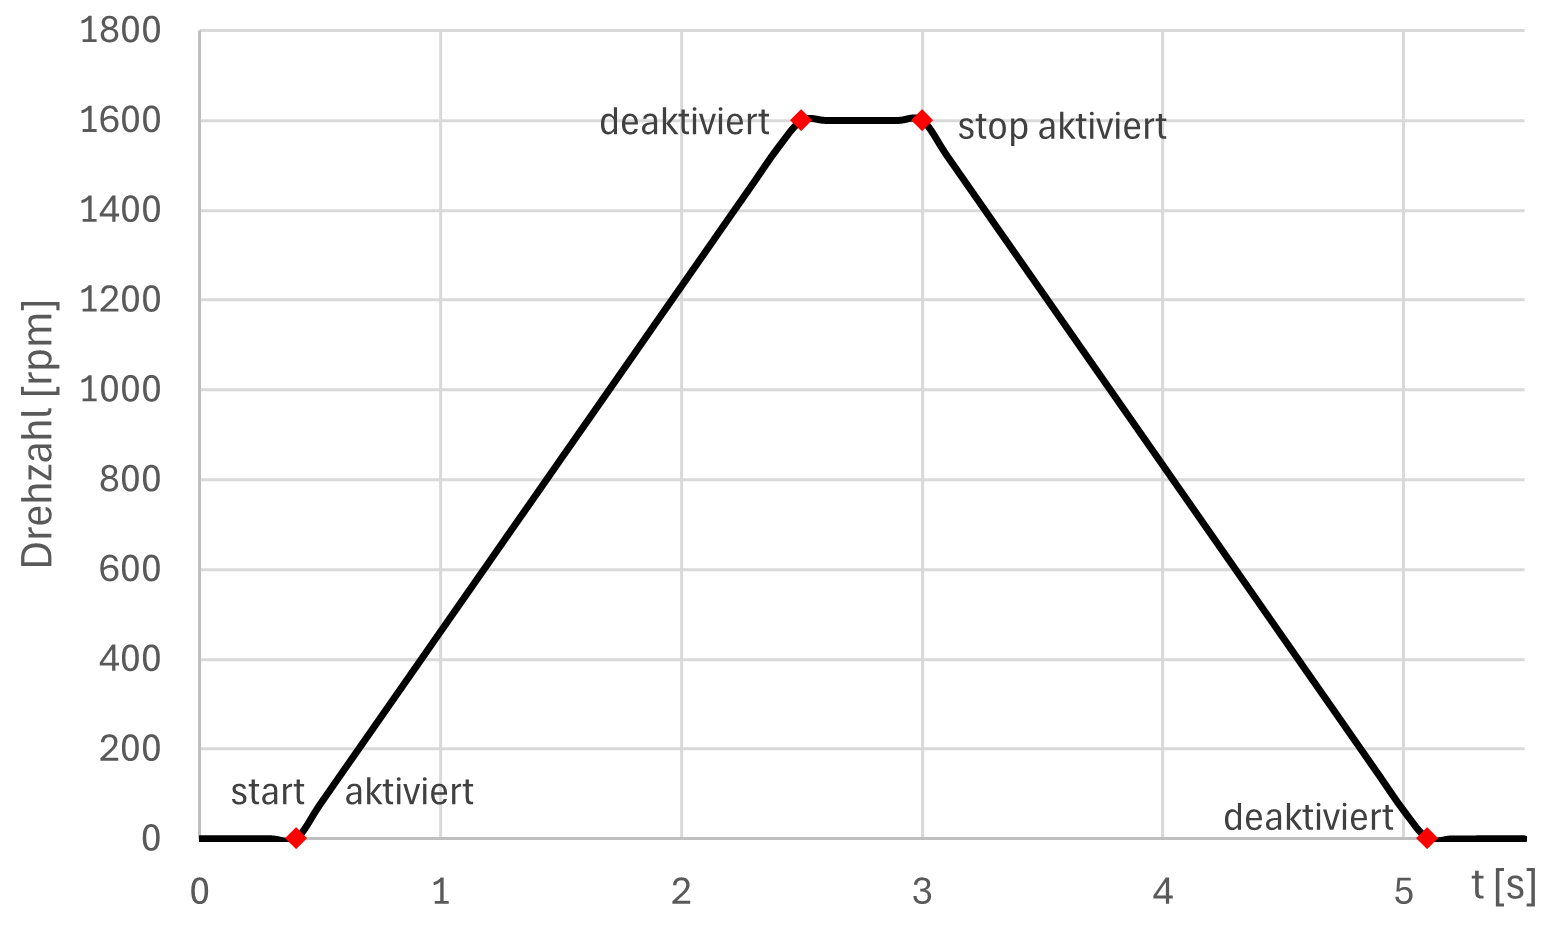
\includegraphics[width=0.75\linewidth]{images/Software/SpeedRamp.png}
	\caption{Drehzahlrampe: Beschleunigen und Bremsen}
	\label{fig:speedRamp}
\end{figure}
\noindent
Die Stopp-Funktion bietet zusätzlich die Möglichkeit über einen booleschen Parameter \verb|immediate| z.B. während einer Notabschaltung den Motor abrupt anzuhalten. In diesem Fall wird nicht die Rampe aktiviert sondern direkt die Motorfunktion \textit{Motor aus} gesetzt. 
\subsection{Steuerung der Linearführung}
nachdem die allgemeine Steuerung des Motors implementiert ist, gilt es, diese auf die Positionierung der Segel über die Linearführung anzuwenden. 
\subsubsection{Kalibrierung}
Damit später eine bestimmte Stellung angefahren werden kann, muss die aktuelle Position jederzeit bekannt sein. Wie bereits erwähnt, dient das Puls-Signal des Motors als Maß, wie weit sich die Position von einem Startpunkt entfernt hat. Jedoch muss dieser Punkt erst angefahren werden, was durch die Detektion der Endschalter keine Schwierigkeit darstellt. Damit kann die absolute Position anhand der Puls-Zahl und der Gewindesteigung ermittelt werden. Für die Einstellung der Segel wird vom Controllino eine Prozentzahl vorgegeben wie weit gerollt oder getrimmt werden soll. Um diesen Wert auf eine absolute Position auf der Linearführung abzubilden, muss zusätzlich die Distanz zwischen den beiden Endpunkten ermittelt werden. Außerdem soll die Grenze zwischen Roll- und Trimmbereich nachträglich manuell angepasst werden können, um potenzielle Asymmetrien in der Seilführung der Segel auszugleichen. Der gesamte Ablauf der Kalibrierung wurde in Form einer Zustandsmaschine realisiert, wie in Abbildung \ref{fig:calibration} dargestellt.
\begin{figure}[H]
	\centering
	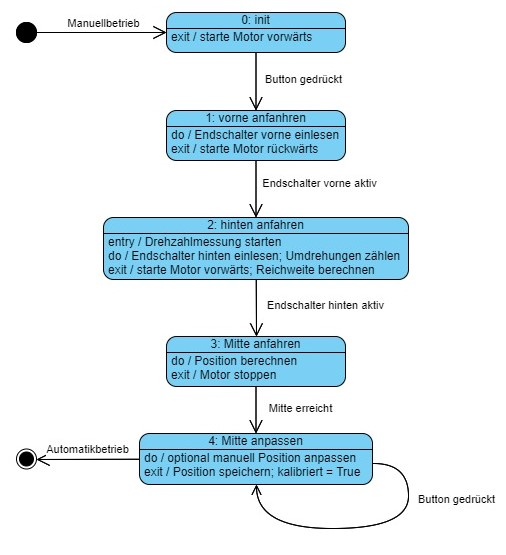
\includegraphics[width=0.8\linewidth]{images/Software/Kalibrierungsprozess.jpg}
	\caption{Kalibrierungsprozess}
	\label{fig:calibration}
\end{figure}
\noindent
Die Eintrittsbedingung der Kalibrierung ist das Einschalten des manuellen Betriebsmodus durch den Kippschalter am Gehäuse oder alternativ über den Webserver. Aus dem Ausgangszustand heraus muss der Knopf \textit{Speichern/Bestätigen} aus Abbildung \ref{fig:Bedienung} gedrückt werden, um die automatische Kalibrierung einzuleiten. Dies ist mit dem starten des Motors in Vorwärtsrichtung und dem Übergang in Zustand 1 verbunden. Anschließend wird der vordere Endschalter abgefragt, bis dieser aktiviert wird und die Endposition erreicht ist. Von dieser Position aus beginnt die Pulszählung, damit nach Ankunft am anderen Ende die zurückgelegte Distanz berechnet werden kann. Aus dieser Distanz wird daraufhin die Mitte bestimmt und angefahren. Ist diese erreicht, kann zuletzt die tatsächliche Grenze manuell über die Knöpfe \textit{Trimmen} und \textit{Rollen} angefahren und mit dem erneuten Druck des einleitenden Knopfes bestätigt werden. Als Feedback blinkt dabei die LED \textit{Position gespeichert}. Ebenso aktivieren bzw. deaktivieren sich nun nach der Einteilung der Bereiche je nach Positionierung die entsprechenden LEDs (\textit{Im Trimmungsbereich} / \textit{Im Rollbereich}).\\
Da die Grenze in Zustand 4 mit dem entsprechenden Knopf beliebig oft angepasst werden kann, ist es durch das selbe Signal nicht möglich, den kompletten Prozess von vorne zu starten, ohne das System neu zu booten. Daher wurde ein Timer mit einem periodischen Callback konfiguriert, der die Dauer des Knopfdrucks ermittelt und ab einer Druckdauer von 3s die Zustandsmaschine zurücksetzt, anstatt lediglich die Grenze zu überschreiben.
\subsubsection{Umsetzung einer Rollung/Trimmung}
\subsubsection{Optimierung der Bewegungsübergänge}
- Berechnung des Bremsweges zum vorzeitigen Bremsen vor Erreichen der Endschalter
- Einführung der gewünschten Position: entspricht bei automatischer Steuerung der Vorgabe und bei manueller Steuerung der Position zum Zeitpunkt des Loslassens der Steuerknöpfe
 - Bremsvorgang mit aktueller Position abgleichen und ggfs. korrigieren
\subsubsection{Wiederherstellung der Position}
1. Teil: FRAM Modul beschreiben...
2. Teil: partielle und vollständige Herstellung der Lokalisierung erklären
\subsubsection{Fehlerbehandlung}
- Windfehler (von Controllino kommuniziert)
	Konsequenz: 100 \% Rollen
- Distanzfehler: Toleranz zwischen Distanzsensor und Puls-Berechnung überschritten?
	Konsequenz: Anpassung der Puls-Zahl anhand Distanzmessung
- Stromfehler: Überstrom an Stromsensor gemessen (Motorstrom)
	Konsequenz: Notabschaltung: abrupter Motorstopp und jeden Steuerbefehl blockieren
- Motorfehler: Fehlerausgang an Motor aktiv
	Konsequenz: Notabschaltung
\subsection{REST Interface}
\subsection{Webserver}





